

%%%%%%%%%%%%%%%%%%%%%%%%
\subsection{Primary Mass}
%%%%%%%%%%%%%%%%%%%%%%%%
\label{subsec:bbh_masses}

In this section, we illustrate the main findings of the strongly and weakly modeled approaches using results from the \BrokenPLTwoPeaks (see Appendix \ref{appendix:BrokenPLTwoPeaks}) and \BSpline (see Appendix \ref{appendix:BSpline}) models, respectively. We chose the \BrokenPLTwoPeaks model as our fiducial mass model because it performed the best in our model comparison study. It was first introduced by \citet{Callister:2023tgi} to describe the \gwtcthree mass distribution. Results from a selection of other models considered in the model comparison study can be found in Appendix \ref{appendix:model_comparison_mass}, while models that employ a \nonparametric can be found in Appendix \ref{appendix:non_parameteric_comparison}, both of which include comparisons to the fiducial \BrokenPLTwoPeaks and \BSpline models. The \parametric employs the default models listed in Table \ref{tab:summary_of_models} for the other source parameters, namely the \powerlawRedshift and \default models.

\textbf{We identify a global peak at $\bm{{\sim}10 \,\Msun}$ and find that it is robust to model variations}. A Gaussian-like peak at ${\sim}10 \,\Msun$ was first identified by \citet{Tiwari:2020otp} and \citet{Edelman:2021zkw} using \gwtctwo and later by the \nonparametrics in \citet{KAGRA:2021duu} using \gwtcthree. Figure \ref{fig:primary_mass_default} shows the rate ${\rm d}\mathcal{R}/{\rm d} m_1$ as a function of primary mass at $z=0.2$ inferred by these models compared to the \PLPeak (see Appendix B of \citealt{KAGRA:2021duu} for a description of this model) inference with \gwtcthree from \citet{KAGRA:2021duu}.\footnote{We quote \ac{BBH} merger rates at $z=0.2$ to be consistent with \citet{KAGRA:2021duu} and because $z\sim0.2$ is where we best constrain the merger rate.} The low-mass Gaussian component of the \BrokenPLTwoPeaks model infers a global peak in the primary mass spectrum at $m_1 = \CIPlusMinus{\defaultbbh[mass_1][peak_1_location]} \,\Msun$ relative to the underlying broken power law continuum. The \BSpline model also recovers a global peak at $m_1 = \CIPlusMinus{\BsplineIID[mass_1][peak_1_location]} \,\Msun$. Both values are consistent with \gwtcthree, which inferred a global peak at $m_1 = $ \muOOT by modeling the mass spectrum as a power law modulated by a spline.

\textbf{A broken power law is necessary to describe the continuum structure above $\bm{{\sim}15 \,\Msun}$} (see Figure \ref{fig:primary_mass_default}). Below ${\sim}35 \, \Msun$, the continuum  of \ac{BH} masses is well described by a power law with spectral index $\alpha_1 = \CIPlusMinus{\defaultbbh[alpha_1]}$. Above ${\sim}35 \, \Msun$, the continuum steepens, with a spectral index of $\alpha_2 = \CIPlusMinus{\defaultbbh[alpha_2]}$ that is consistent with the \PLPeak result from \gwtcthree ($\alpha = $ \alphaOT). We find that $\alpha_2 > \alpha_1$ at $\defaultbbh[alpha_diff_perc] \%$ credibility. Though this continuum structure was identified by \citet{Callister:2023tgi}, it was not identified by the \parametrics in \citet{KAGRA:2021duu}, in part due to the limited flexibility of models employed in \citet{KAGRA:2021duu}. To illustrate this, in Figure \ref{fig:primary_mass_o3b_comparison} we present a re-analysis of \gwtcthree using the \BrokenPLTwoPeaks model alongside the \gwtcfour result, which shows improved constraints across the full mass spectrum. 

\textbf{We identify a feature at $\bm{{\sim}35\, \Msun}$}. Using the \parametric, we find that this feature is consistent with either: (i) an over-density that peaks at $m_1 = \CIPlusMinus{\defaultbbh[mass_1][peak_2_location]} \, \Msun$ relative to an underlying broken power law (i.e., the \BrokenPLTwoPeaks result), or (ii) a broken power law with break mass $m_\text{break} = \CIPlusMinus{\PowerLawTwoPeakOneBBH[break_mass]} \,\Msun$ (i.e., a broken power law without a second peak near the break). See Appendix \ref{appendix:model_comparison_mass} for a more detailed discussion of this result. The former conclusion is supported by the \BSpline model, which exhibits a local peak at $m_1 = \CIPlusMinus{\BsplineIID[mass_1][peak_2_location]} \,\Msun$, consistent with other models that employ a \nonparametric in Appendix \ref{appendix:non_parameteric_comparison}. 

\textbf{Additional structure may be present in the mass spectrum}. A bump near ${\sim}20 \,\Msun$ is present in some of the \nonparametrics (see Figure \ref{fig:bbh_mass_non_parametrics} in Appendix \ref{appendix:non_parameteric_comparison}). We cannot conclude with the \parametric whether adding a third Gaussian component to the \BrokenPLTwoPeaks model in this region is required by the data or not (as quantified by the log Bayes factor $\log_{10}\mathcal{B} = \BBHMassModelBayesFactors[pl2pk3]$ between the default model and one including a third peak). This feature was first reported in an analysis of \gwtctwo \citep{Tiwari:2020otp} and was present in several analyses of \gwtcthree \citep{KAGRA:2021duu,Edelman:2022ydv, Tiwari:2023xff,Godfrey:2023oxb}. Additionally, the \BSpline and other \nonparametrics show a rise in the merger rate relative to the \BrokenPLTwoPeaks result in the ${\sim}60 \,\Msun$ region, which can be seen in Figure \ref{fig:primary_mass_default} and Figure \ref{fig:bbh_mass_non_parametrics}. A previous study of \gwtcthree found evidence for a similar feature in this region \citep{MaganaHernandez:2024qkz}.


\begin{figure*}[t]
	\centering
	\includegraphics[width=0.9\linewidth]{figures/fig_primary_mass_default_comparison.pdf}
	\caption{Differential merger rate as a function of primary mass (evaluated at $z=0.2$) of the \BrokenPLTwoPeaks model inferred with \gwtcfour compared to the same model applied to only \gwtcthree \ac{BBH} events. The orange shaded region shows the 90\% credible interval for \gwtcfour and the solid orange curve shows the posterior median, while the black dashed curves bound the $90\%$ credible region for \gwtcthree and the solid black curve shows the posterior median. The inferred distribution is similar between catalogs, which highlights that the low-mass structure identified in \gwtcfour was present in \gwtcthree. The inset figure shows the joint posterior of the broken power law index parameters $\alpha_1$ and $\alpha_2$ for \gwtcthree (gray) and \gwtcfour (orange), with the contours showing the $5^{\rm th}, 50^{\rm th}$, and $95^{\rm th}$ percentiles. The black dashed curve in the inset indicates where $\alpha_1 = \alpha_2$.}
	\label{fig:primary_mass_o3b_comparison}
  \end{figure*}

We do not place informative constraints on the individual parameters that govern low-mass smoothing for the \BrokenPLTwoPeaks model. We caution against astrophysically interpreting the \ac{BBH} primary mass distribution below ${\sim} 8 \,\Msun$ because of the bias that may be introduced by removing the probable \ac{NS}-containing events in the manner described in Section~\ref{sec:data}. Removing such events is responsible for the discrepancy below ${\sim} 8 \,\Msun$ between Figure \ref{fig:full_mass_spectrum} and Figure \ref{fig:primary_mass_default}.

\gwtcfour includes an exceptional high-mass BBH, GW231123~\citep{GW231123}, whose inferred component masses lie at the extreme upper end of those in our dataset. To check if GW231123 is an outlier with respect to the mass distribution of \acp{BBH}, we construct mock catalogs containing $153$ detected events following the inferred population without GW231123, and calculate the distribution of maximum detectable \ac{BH} masses. The total mass of GW231123 lies at the $\CIPlusMinus{\OutlierTestMassiveEvent[percentilemmax300][total_mass_source]}$th percentile of this distribution. This shows that while GW231123 lies in the tail of the distribution, its total mass is consistent with the inferred mass spectrum; the degree of consistency is more than was the case with \gwtcthree data alone~\citep{GW231123}.

The main compact binary formation scenarios (\citealt{{Mandel:2018hfr}} and references therein)---isolated binary evolution and dynamical assembly in dense stellar environments---have both been shown to produce populations consistent with current observations \citep{Mandel:2021smh}. A peak near $m_1 \sim 10 \, \Msun$ is often predicted by isolated binary evolution models \citep{Dominik:2014yma, Belczynski:2017gds, Giacobbo:2018etu, Wiktorowicz:2019dil, Neijssel:2019irh}, while mass distributions from dynamical formation, such as in young and globular clusters, typically peak above $10\, \Msun$ \citep{Rodriguez:2016kxx, Hong:2018bqs, Rodriguez:2019huv, Banerjee:2020qub, Antonini:2020xnd}. However, predictions from isolated and dynamical formation often overlap and can vary significantly based on the assumptions and methodologies used, making it difficult to conclude the origin of the observed catalog or constrain formation physics based on features in the marginal mass distributions. 

A feature that may provide distinguishing power between the isolated and dynamical channels is the existence of an upper mass gap, in the range $45\,\Msun \lesssim m \lesssim 120 \,\Msun$. Such a dearth would be consistent with the theorized \textit{pair-instability mass gap}, arising from the complete disruption of massive stars due to runaway electron--positron pair production \citep{Woosley:2016hmi,Mapelli:2019ipt,Farmer:2019jed}. While the precise locations of the lower and upper edges of the pair-instability mass gap are sensitive to physical assumptions \citep{Renzo:2020rzx, vanSon:2020zbk, Woosley:2021xba, Shen:2023rco, Winch:2024xdt}, the feature tends to be a robust prediction of most stellar evolution models \citep{Marchant:2018kun,Marchant:2020haw,Renzo:2020rzx,Woosley:2021xba}. The gap may not be completely empty due to overmassive stellar envelope fallback or stellar mergers \citep{DiCarlo:2019pmf, DiCarlo:2019fcq, Mapelli:2019ipt, Kremer:2020wtp}, hierarchical BBH mergers in clusters or in AGN environments \citep{Mckernan:2017ssq, Rodriguez:2019huv, McKernan:2019beu, Yang:2019okq, Mapelli:2020xeq, Antonini:2018auk, Fragione:2020nib, Liu:2020gif, Martinez:2020lzt, Sedda:2020jvg, Mahapatra:2021hme, Mahapatra:2022ngs, Mahapatra:2024qsy}, or even due to primordial \acp{BH} \citep{Postnov:2014tza, Bird:2016dcv, Clesse:2020ghq}. The decrease in the merger rate above $m_1 \sim35 \, \Msun$ seen in all models and the tentative rise near $m_1\sim60 \, \Msun$ seen in the \nonparametrics may hint toward a polluted mass gap.


\begin{figure}
	\centering
	\includegraphics[width=0.9\columnwidth]{figures/mass_ratio_default.pdf}
	\caption{Differential merger rate as a function of mass-ratio (evaluated at $z=0.2$) of the \BrokenPLTwoPeaks model (orange) and \BSpline model (blue). The fiducial \textsc{Power Law + Peak} model from \citet{KAGRA:2021duu} is included for comparison. Solid curves indicate posterior medians and the shaded (dashed) regions show 90\% credible intervals.}
	\label{fig:mass_ratio_default}
  \end{figure}


\subsection{Mass-Ratio}
\label{subsec:bbh_ratio}

Figure \ref{fig:mass_ratio_default} shows the differential merger rate ${\rm d}\mathcal{R}/{\rm d}q$ evaluated at $z = 0.2$ inferred by the \BrokenPLTwoPeaks and \BSpline models compared to the \PLPeak result from \gwtcthree.\footnote{Models that utilize B-Splines infer the separable distribution $p(q)$ but the results of such models shown in this section are actually the conditional marginal distribution $p(q|m_2{>}3\Msun)$. See Appendix \ref{appendix:BSpline} for further details.}

\textbf{We find that the mass-ratio distribution can be described by a power-law with an index $\bm{\beta_q = \CIPlusMinus{\defaultbbh[beta]}}$} that is consistent with \gwtcthree ($\beta_q = 1.1^{+1.7}_{-1.3}$) with a reduction in uncertainty. The \BSpline model shows a reduced rate above $q \gtrsim 0.8$ relative to the \BrokenPLTwoPeaks result. More flexible parametrizations in the \parametric were explored (see also the other \nonparametrics in Figure \ref{fig:bbh_mass_non_parametrics}, which do peak near unity), but model comparisons were inconclusive. Similarly, in \gwtcthree, \citet{Godfrey:2023oxb} inferred a mass-ratio distribution peaked away from unity using a \nonparametric, while \citet{Rinaldi:2025emt} found equal evidence for two \parametrics with very distinct behavior above $q \gtrsim 0.7$. 

Models that incorporate correlations between source parameters have a greater potential to distinguish between formation channels than uncorrelated ones. We next present results from two different models that correlate features of the primary mass spectrum with different mass-ratio distributions. 

\textbf{\acp{BH} with masses $\bm{{\sim} 35\, \Msun}$ preferentially merge with other \acp{BH} of more equal mass relative to those in the underlying mass continuum.} The \ExtendedBrokenPLTwoPeaks model modifies the \BrokenPLTwoPeaks model by allowing each primary mass mixture component (i.e., the broken power law and two Gaussian components) to be associated with a different power-law-mass-ratio distribution. Figure \ref{fig:mass_ratio_peak} shows the mass-ratio distribution for each mixture component. Specifically, each component infers a different power-law index $\beta_q$, with $\beta_q^{\rm BP} = \CIPlusMinus{\VaryingBetaQsDominantMode[param][beta_q_power_law]}$ for the broken power law, $\beta_q^{\rm peak1} = \CIPlusMinus{\VaryingBetaQsDominantMode[param][beta_q_low_mass_peak]}$ for the Gaussian component that captures the ${\sim}10\, \Msun$ peak, and $\beta_q^{\rm peak2} = \CIPlusMinus{\VaryingBetaQsDominantMode[param][beta_q_high_mass_peak]}$ for the second Gaussian component that captures the ${\sim}35 \, \Msun$ feature. Critically, $\beta_q^{\rm peak2} > \beta_q^{\rm BP}$ at $\VaryingBetaQsDominantModeBetaDiffPerc[beta_peak_pl_diff_perc] \%$ credibility. See Appendix \ref{appendix:model_comparison_mass} for a more detailed discussion of this result. Other studies of \gwtcthree have drawn similar conclusions about the pairing preferences of high mass \acp{BH} \citep[e.g., ][]{Li:2022jge, Baibhav:2022qxm, Sadiq:2023zee, Galaudage:2024meo, Roy:2025ktr}. 

\textbf{\acp{BH} with masses $\bm{{\sim}10\, \Msun}$ may prefentially merge with lighter \acp{BH}}. The region bounded by the solid blue curves in the bottom panel of Figure \ref{fig:mass_ratio_peak} shows the mass-ratio distribution of the ${\sim}10 \,\Msun$ peak inferred with the \textsc{Isolated Peak} model. This model is a mixture of a Gaussian peak and a B-Spline (continuum) in primary mass, and the mass ratio and spin distributions are inferred separately for each mixture component with B-Splines (see Appendix \ref{appendix:non_parametric_models_summary} for further details). The Gaussain peak is inferred at ${\sim}10 \,\Msun$ and its mass-ratio distribution exhibits a peak at $q = \CIPlusMinus{\IsoPeakIID[mass_ratio][peak][peak_location]}$, a feature that a single power law is unable to reproduce. This could explain the large uncertainty in $\beta_q^{\rm peak1}$ from the \ExtendedBrokenPLTwoPeaks model. The solid blue curve in Figure \ref{fig:mass_ratio_peak} shows the mass-ratio distribution of masses outside of the ${\sim}10 \,\Msun$ peak inferred by the B-Spline mixture component. Unlike the full population mass-ratio distribution inferred by the \BSpline model in Figure \ref{fig:mass_ratio_default}, this result does not possess a peak near $q \sim 0.8$, indicating that the peak seen in the full population is due largely to the events around ${\sim}10 \,\Msun$. This mass feature was identified in \gwtcthree by \citet{Godfrey:2023oxb}. 

\begin{figure}[t]
	\centering
	  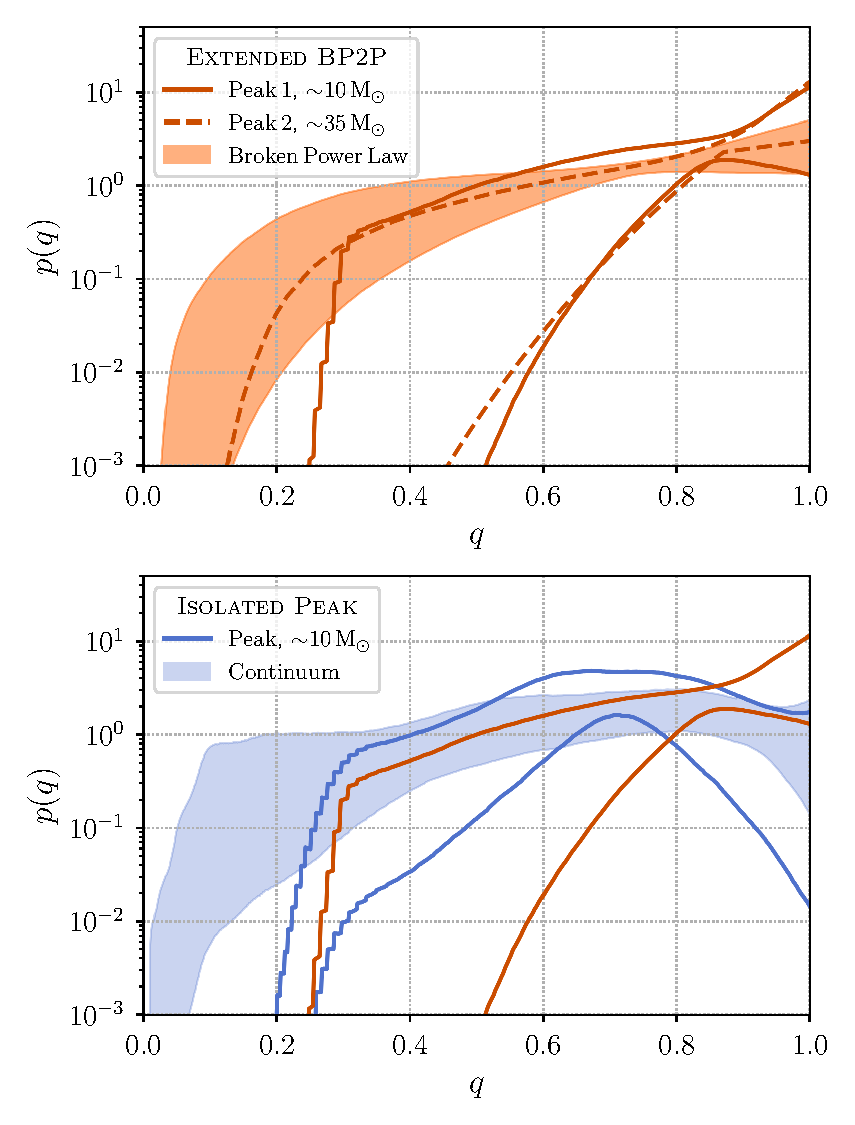
\includegraphics[width=0.6\columnwidth]{figures/fig_mass_ratio_peak.pdf}
	  \caption{Top Panel: The $90\%$ credible regions for the mass-ratio distribution of the ${\sim}10 \,\Msun$ peak (solid orange curves), ${\sim}35 \,\Msun$ peak (dashed curves), and continuum (orange shaded region) components of the \ExtendedBrokenPLTwoPeaks model. Bottom Panel: The $90\%$ credible regions for mass-ratio distribution of the ${\sim}10 \,\Msun$ peak (solid blue curves) and the rest of the mass spectrum (blue shaded region) inferred with the \textsc{Isolated Peak} model. The ${\sim}10\, \Msun$ peak mass-ratio distribution from the \ExtendedBrokenPLTwoPeaks is included for comparison.}
	  \label{fig:mass_ratio_peak}
  \end{figure}

Most formation channels generally favor equal mass systems. For example, dynamical formation can produce systems with a wide range of mass ratios, but predicted distributions typically peak at unity \citep{Rodriguez:2016kxx, Torniamenti:2024uxl}. Certain hierarchical mergers may not necessarily follow this trend, in particular mergers between first generation and second generation BHs have been shown to produce a mass-ratio distribution peaked near $q \sim 0.5$ \citep{Rodriguez:2019huv}. Mass transfer during the contact phase of binaries formed via chemically homogeneous evolution~\citep{deMink:2016vkw, Marchant:2016wow} leads to a strong preference for equal mass-ratio systems, but this mechanism is thought to be important for binaries with $\massone \gtrsim 10\,\Msun$~\citep{duBuisson:2020asn, Zevin:2020gbd, Riley:2020btf}. Mass-ratio reversal within the stable mass transfer channel can lead to a peak in the mass-ratio distribution between $q\sim$ 0.6-0.8 \citep{Neijssel:2019irh,vanSon:2021zpk}, which is qualitatively consistent with the mass-ratio distribution of the ${\sim}10 \,\Msun$ inferred with the \textsc{Isolated Peak} model. Stable mass transfer also predicts a peak near ${\sim}10 \,\Msun$ that is robust to uncertainties in the metallicity-dependent star formation history \citep{vanSon:2022ylf} and other physical uncertainties of the channel \citep{vanSon:2022myr}.